% ------------------------------------------------------------------------------
% TYPO3 CMS 8 LTS - What's New - Chapter "Deprecated Functions" (English Version)
%
% @author	Michael Schams <schams.net>
% @license	Creative Commons BY-NC-SA 3.0
% @link		http://typo3.org/download/release-notes/whats-new/
% @language	English
% ------------------------------------------------------------------------------
% LTXE-CHAPTER-UID:		3f842373-9262b8d3-f9c8de76-cf29ce17
% LTXE-CHAPTER-NAME:	Deprecated Functions
% ------------------------------------------------------------------------------

\section{Deprecated/Removed Functions}
\begin{frame}[fragile]
	\frametitle{Deprecated/Removed Functions}

	\begin{center}\huge{\color{typo3darkgrey}\textbf{Deprecated/Removed Functions}}\end{center}
	\begin{center}\large{\textit{}}\end{center}

\end{frame}

% ------------------------------------------------------------------------------
% LTXE-SLIDE-START
% LTXE-SLIDE-UID:		d4c8c340-33163839-2ae654ee-9c6834da
% LTXE-SLIDE-TITLE:		Miscellaneous (#72337, #75150 and #73794)
% ------------------------------------------------------------------------------

\begin{frame}[fragile]
	\frametitle{Deprecated/Removed Functions}
	\framesubtitle{Miscellaneous}

	\begin{itemize}

		\item The following configuration options have been removed:

			\begin{itemize}
				\item \texttt{\$TYPO3\_CONF\_VARS['SYS']['t3lib\_cs\_utils']}
				\item \texttt{\$TYPO3\_CONF\_VARS['SYS']['t3lib\_cs\_convMethod']}
			\end{itemize}

			\small
				(functionality is now auto-detected and \texttt{mbstring} is
				used by default if available)
			\normalsize

		\item The deprecated TypoScript property \texttt{page.includeJSlibs} has
			been removed. Use the TypoScript property \texttt{page.includeJSLibs}
			(capital "L") instead

		\item The TypoScript option \texttt{config.renderCharset}, which was used
			as character set for internal conversion within a frontend request,
			has been removed

	\end{itemize}

\end{frame}

% ------------------------------------------------------------------------------
% LTXE-SLIDE-START
% LTXE-SLIDE-UID:		dfff0a4a-601e8cb2-abb7af47-f9861736
% LTXE-SLIDE-TITLE:		#70056: Curl and HttpRequest removed (1)
% ------------------------------------------------------------------------------

\begin{frame}[fragile]
	\frametitle{Deprecated/Removed Functions}
	\framesubtitle{Http-related Options and HttpRequest Class Removed (1)}

	\begin{itemize}

		\item The following PHP classes have been \textbf{removed}:

			\begin{itemize}
				\item \small\texttt{
					TYPO3\textbackslash
					CMS\textbackslash
					Core\textbackslash
					Http\textbackslash
					HttpRequest}\normalsize
				\item \small\texttt{
					TYPO3\textbackslash
					CMS\textbackslash
					Core\textbackslash
					Http\textbackslash
					Observer\textbackslash
					Download}\normalsize
			\end{itemize}

		\item The following options have been \textbf{renamed}:

			\begin{itemize}

				\item
					\small
						old:\tabto{1cm}\texttt{\$TYPO3\_CONF\_VARS[HTTP][userAgent]}\newline
						new:\tabto{1cm}\texttt{\$TYPO3\_CONF\_VARS[HTTP][headers][User-Agent]}

				\item
					\small
						old:\tabto{1cm}\texttt{\$TYPO3\_CONF\_VARS[HTTP][protocol\_version]}\newline
						new:\tabto{1cm}\texttt{\$TYPO3\_CONF\_VARS[HTTP][version]}

			\end{itemize}

	\end{itemize}

\end{frame}

% ------------------------------------------------------------------------------
% LTXE-SLIDE-START
% LTXE-SLIDE-UID:		ed21f1c2-5d947af5-9d35c427-05dfcf48
% LTXE-SLIDE-TITLE:		#70056: Curl and HttpRequest removed (2)
% ------------------------------------------------------------------------------

\begin{frame}[fragile]
	\frametitle{Deprecated/Removed Functions}
	\framesubtitle{Http-related Options and HttpRequest Class Removed (2)}

	\begin{itemize}

		\item All proxy-related options are unified within\newline
			\small\texttt{\$TYPO3\_CONF\_VARS[HTTP][proxy]}\normalsize

		\item All redirect-related options
			(\small
				\texttt{HTTP/follow\_redirects},
				\texttt{HTTP/max\_redirects},
				\texttt{HTTP/strict\_redirects}\normalsize)
			are unified within
			\small
				\texttt{\$TYPO3\_CONF\_VARS[HTTP][allow\_redirects]}
			\normalsize

		\item All options related to SSL private keys
			(\small
				\texttt{HTTP/ssl\_local\_cert},
				\texttt{HTTP/ssl\_passphrase}\normalsize)
			are merged into
			\small
				\texttt{\$TYPO3\_CONF\_VARS[HTTP][ssl\_key]}
			\normalsize

		\item All options related to verify SSL peers are merged into
			\small
				\texttt{\$TYPO3\_CONF\_VARS[HTTP][verify]}
			\normalsize

	\end{itemize}

\end{frame}

% ------------------------------------------------------------------------------
% LTXE-SLIDE-START
% LTXE-SLIDE-UID:		ab377e1e-884fa3e4-74a17b45-77aa66c0
% LTXE-SLIDE-TITLE:		[ExtJS Removal 1] #78521: Drop unused JavaScript from backend.js
% ------------------------------------------------------------------------------
\begin{frame}[fragile]
	\frametitle{Deprecated/Removed Functions}
	\framesubtitle{ExtJS Removal (1)}

	\begin{itemize}
		\item As part of the ExtJS removal work package, the following JavaScript methods have been removed
			from the Backend main frame (defined in file \texttt{backend.js}):

		\begin{itemize}
			\item \texttt{TYPO3.\_instances}
			\item \texttt{TYPO3.addInstance}
			\item \texttt{TYPO3.getInstance}
			\item \texttt{TYPO3.helpers.split}
		\end{itemize}

	\end{itemize}

\end{frame}
% ------------------------------------------------------------------------------
% LTXE-SLIDE-START
% LTXE-SLIDE-UID:		58f2f5e1-778a1dff-969667d4-aa4c3e7b
% LTXE-SLIDE-TITLE:		[ExtJS Removal 2] #78468: Remove ExtDirect from EXT:workspaces
% ------------------------------------------------------------------------------
\begin{frame}[fragile]
	\frametitle{Deprecated/Removed Functions}
	\framesubtitle{ExtJS Removal (2)}

	\begin{itemize}
		\item New class
			\texttt{TYPO3\textbackslash
				CMS\textbackslash
				Workspaces\textbackslash
				Controller\textbackslash
				AjaxDispatcher}
			replaces the ExtDirect router functionality in \texttt{EXT:workspaces}

		\item The following classes have been moved:

		\begin{itemize}
			\item \smaller\texttt{Classes/ExtDirect/AbstractHandler.php}\newline
				now as: \texttt{Classes/Controller/Remote/AbstractHandler.php}\normalsize

			\item \smaller\texttt{Classes/ExtDirect/ActionHandler.php}\newline
				now as: \texttt{Classes/Controller/Remote/ActionHandler.php}\normalsize

			\item \smaller\texttt{Classes/ExtDirect/MassActionHandler.php}\newline
				now as: \texttt{Classes/Controller/Remote/MassActionHandler.php}\normalsize

			\item \smaller\texttt{Classes/ExtDirect/ExtDirectServer.php}\newline
				now as: \texttt{Classes/Controller/Remote/RemoteServer.php}\normalsize

		\end{itemize}

	\end{itemize}

\end{frame}
% ------------------------------------------------------------------------------
% LTXE-SLIDE-START
% LTXE-SLIDE-UID:		877e457d-ab15dfaa-85e46a57-335dc6a3
% LTXE-SLIDE-TITLE:		#78244: TYPO3_DB and Prepared Statement classes are deprecated
% ------------------------------------------------------------------------------
\begin{frame}[fragile]
	\frametitle{Deprecated/Removed Fasunctions}
	\framesubtitle{Classes \texttt{DatabaseConnection} and \texttt{PreparedStatement}}

	\begin{itemize}
		\item The following classes have been marked as \textit{deprecated}:
			\begin{itemize}
				\item \texttt{TYPO3\textbackslash
						CMS\textbackslash
						Core\textbackslash
						Database\textbackslash
						DatabaseConnection}
				\item \texttt{TYPO3\textbackslash
						CMS\textbackslash
						Core\textbackslash
						Database\textbackslash
						PreparedStatement}
			\end{itemize}
		\item Use Doctrine DBAL in TYPO3 v8 LTS instead\newline
				(\texttt{ConnectionPool} and \texttt{QueryBuilder} classes)
		\item These two classes will be removed in TYPO3 v9
	\end{itemize}

\end{frame}


% ------------------------------------------------------------------------------
% LTXE-SLIDE-START
% LTXE-SLIDE-UID:		70f29777-68968704-618a9b16-3bf2eea2
% LTXE-SLIDE-TITLE:		#78522 and #78525: JavaScript settings under TYPO3.configuration
% ------------------------------------------------------------------------------
\begin{frame}[fragile]
	\frametitle{Deprecated/Removed Functions}
	\framesubtitle{JavaScript settings under \texttt{TYPO3.configuration}}

	\begin{itemize}
		\item The following JavaScript settings have been removed:

		\begin{itemize}
			\item \texttt{TYPO3.configuration.debugInWindow}
			\item \texttt{TYPO3.configuration.moduleMenuWidth}
			\item \texttt{TYPO3.configuration.topBarHeight}
		\end{itemize}

		\item These options were not used by the TYPO3 core anyway

	\end{itemize}

\end{frame}


% ------------------------------------------------------------------------------
% LTXE-SLIDE-START
% LTXE-SLIDE-UID:		7e836e1e-3132a797-0f3a0c68-88037011
% LTXE-SLIDE-TITLE:		#78581: FlexFormTools public properties dropped
% ------------------------------------------------------------------------------
\begin{frame}[fragile]
	\frametitle{Deprecated/Removed Functions}
	\framesubtitle{Public Properties of \texttt{FlexFormTools}}

	\begin{itemize}
		\item Two public properties have been dropped from class
			\texttt{TYPO3\textbackslash
				CMS\textbackslash
				Core\textbackslash
				Configuration\textbackslash
				FlexForm\textbackslash
				FlexFormTools}:

		\begin{itemize}
			\item \texttt{public \$traverseFlexFormXMLData\_DS = array();}
			\item \texttt{public \$traverseFlexFormXMLData\_Data = array();}
		\end{itemize}

		\item Accessing those properties will throw a warning now

	\end{itemize}

\end{frame}




% ------------------------------------------------------------------------------
% LTXE-SLIDE-START
% LTXE-SLIDE-UID:		82f525e3-eddc6639-96053da3-bc74d15b
% LTXE-SLIDE-TITLE:		#78217: frameset and frame
% ------------------------------------------------------------------------------
\begin{frame}[fragile]
	\frametitle{Deprecated/Removed Functions}
	\framesubtitle{Frameset and frame}

	\begin{itemize}
		\item \texttt{frameset} and \texttt{frame} are not supported in HTML5 anymore
		\item The following TypoScript objects have been marked as \textit{deprecated}:

			\begin{itemize}
				\item \texttt{frameset}
				\item \texttt{frame}
			\end{itemize}

		\item The following TypoScript options have been marked as \textit{deprecated}:

			\begin{itemize}
				\item \texttt{config.frameReloadIfNotInFrameset}
				\item \texttt{config.doctype = xhtml\_frames}
				\item \texttt{config.xhtmlDoctype = xhtml\_frames}
				\item \texttt{frameSet} \tabto{1.8cm}\textit{(and its options)}
				\item \texttt{FRAME} \tabto{1.8cm}\textit{(and its options)}
				\item \texttt{FRAMESET} \tabto{1.8cm}\textit{(and its options)}
			\end{itemize}

	\end{itemize}

\end{frame}

% ------------------------------------------------------------------------------
% LTXE-SLIDE-START
% LTXE-SLIDE-UID:		1b162dfa-75daabe7-fa50f9d2-a6be83d3
% LTXE-SLIDE-TITLE:		!Breaking: #77460 - Extbase query cache removed
% LTXE-SLIDE-REFERENCE:	!Breaking-77460-ExtbaseQueryCacheRemoved.rst
% ------------------------------------------------------------------------------
\begin{frame}[fragile]
	\frametitle{Deprecated/Removed Functions}
	\framesubtitle{Extbase Query Cache Removed}

	\begin{itemize}

		\item The PHP-based query cache functionality within the Extbase persistence layer has been removed

		\item The following public methods within the Extbase persistence layer have been removed:

			\begin{itemize}
				\item \small\texttt{Typo3DbBackend->quoteTextValueCallback()}\normalsize
				\item \small\texttt{Typo3DbBackend->injectCacheManager()}\normalsize
				\item Interface definition in \small\texttt{QuerySettingsInterface->getUseQueryCache}\normalsize
			\end{itemize}

		\item The according cache configuration has no effect anymore:\newline
			\smaller
				\texttt{\$TYPO3\_CONF\_VARS[SYS][cache][cacheConfigurations]}\newline
				\tabto{0.4cm}\texttt{[extbase\_typo3dbbackend\_queries]}
			\normalsize

	\end{itemize}

\end{frame}

% ------------------------------------------------------------------------------
% LTXE-SLIDE-START
% LTXE-SLIDE-UID:		17027d66-b0c438e9-772bb37e-87c9da9e
% LTXE-SLIDE-TITLE:		!Deprecation: #77432 - Extbase: Prepared Statement Query Option
% LTXE-SLIDE-REFERENCE:	!Deprecation-77432-ExtbasePreparedStatementQueryOption.rst
% ------------------------------------------------------------------------------

\begin{frame}[fragile]
	\frametitle{Deprecated/Removed Functions}
	\framesubtitle{Extbase: Prepared Statement Query Option}

	\begin{itemize}

		\item The option to use prepared statements within the Extbase persistence has been removed

		\item The following methods have been removed from the \texttt{QuerySettingsInterface},
			as the database abstraction layer will take care of prepared statements automatically:

			\begin{itemize}
				\item \texttt{getUsePreparedStatement()}
				\item \texttt{usePreparedStatement()}
			\end{itemize}

	\end{itemize}

\end{frame}

% ------------------------------------------------------------------------------
% LTXE-SLIDE-START
% LTXE-SLIDE-UID:		e9bd05a6-e4bff973-742f35ac-bb5a483c
% LTXE-SLIDE-TITLE:		Miscellaneous (3)
% ------------------------------------------------------------------------------
\begin{frame}[fragile]
	\frametitle{Deprecated/Removed Functions}
	\framesubtitle{Miscellaneous (3)}

	% #78279: Deprecate top.TYPO3.Backend.ContentContainer.iframe
	% #78628: TCA tree pageTsConfig addItems icon path
	% #78647: (EXT:lang) language files moved to Resources/Private/Language/

	\begin{itemize}

		\item The following TCA option has been removed:\newline
			\texttt{\$TCA[\$table][ctrl][versioning\_followPages]}

		\item Adding items to TCA tree with pageTsConfig \texttt{addItems} requires an icon identifiers
			from the icon registry now (paths are not supported anymore):\newline
			\smaller
				\texttt{TCEFORM.pages.category.addItems.12345.icon = my-registered-icon}
			\normalsize

		\item \underline{All} XLIF Language files of EXT:lang have been moved to\newline
			\texttt{Resources/Private/Language/}\newline
			This affects all extensions which use labels from EXT:lang!\newline
			\smaller
				OLD: \texttt{EXT:lang/locallang\_alt\_doc.xlf}\newline
				NEW: \texttt{EXT:lang/Resources/Private/Language/locallang\_alt\_doc.xlf}
			\normalsize

	\end{itemize}

\end{frame}

% ------------------------------------------------------------------------------
% LTXE-SLIDE-START
% LTXE-SLIDE-UID:		f0fb603c-54e9f255-03140395-b6b18103
% LTXE-SLIDE-TITLE:		#78384: Frontend ignores TCA in ext_tables.php
% ------------------------------------------------------------------------------
\begin{frame}[fragile]
	\frametitle{In-Depth Changes}
	\framesubtitle{TCA in \texttt{ext\_tables.php}}

	\begin{itemize}
		\item Frontend requests no longer load \texttt{ext\_tables.php} in requests
		\item This change impacts extensions which configure the TCA in \texttt{ext\_tables.php}\newline
			\small(which is not allowed anyway)\normalsize
		\item Install Tool provides a test "TCA ext\_tables check" to identify such extensions
	\end{itemize}

	\begin{figure}
		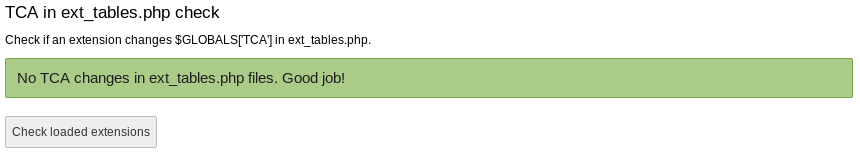
\includegraphics[width=0.95\linewidth]{DeprecatedRemovedFunctions/78384-install-tool-tca-in-exttables-check.png}
	\end{figure}

\end{frame}

% ------------------------------------------------------------------------------
% LTXE-SLIDE-START
% LTXE-SLIDE-UID:		91358547-99cab1b1-208f0f24-a5737bee
% LTXE-SLIDE-TITLE:		Removal of Fluid Styled Content Menu ViewHelpers (1/3)
% LTXE-SLIDE-REFERENCE:	!Breaking: #79622 - Removal of Fluid Styled Content Menu ViewHelpers
% ------------------------------------------------------------------------------

\begin{frame}[fragile]
	\frametitle{Extbase \& Fluid}
	\framesubtitle{Removal of Fluid Styled Content Menu ViewHelpers (1/3)}

	\begin{itemize}
		\item Fetching data directly in the view is not recommended and
			the temporary solution of menu ViewHelpers has been replaced by
			its successor, the menu processor that is based on HMENU.

		\item Menu ViewHelpers have been moved to the \texttt{compatibility7}
			extension, and are replaced in the core menu content elements.

	\end{itemize}

\end{frame}

% ------------------------------------------------------------------------------
